\textbf{Introduction}
The purpose of this test was to see if the GPS coordinates was spoofed correctly and read probably by AQ and to validate the ROS node responsible for creating CAN messages was working as long as the drone is laying on a table. If this works, it shows that the UKF works with the spoofed coordinates as expected, and that the author of the report can spoof the GPS position from a vision based localization system. \\

A rosbag was used to collect data from the GPS since it publishes data to a topic when played as a node did when the recording took place. This results in no code has to be written and when the code works with a rosbag it also works when it is replaced with a node providing real-world data. \\

\textbf{Test}
\begin{figure}[H]
    \center
    \includegraphics[width=0.8\textwidth]{graphics/Indoore_test_spoofed_can.png}
    \caption{Block schematic of the connected components}
    \label{fig:test_block}
\end{figure}


Figure\ref{fig:test_block} shows the connected componenets. 


To get the NMEA strings from the GPS, an already existing Frobomind component will be used. It reads from a serial port, and publishes the parsed NMEA string to \textit{/fmData/nmea\_from\_gps}. Rosbag was then used to save the messages.
The code written by the author will then subscribe to \textit{/fmData/nmea\_from\_gps} and publish the CAN-messages to another topic. A third node which is also a part of Frobomind will then subscribe and send the CAN-messages.

\begin{figure}[H]
    \center
    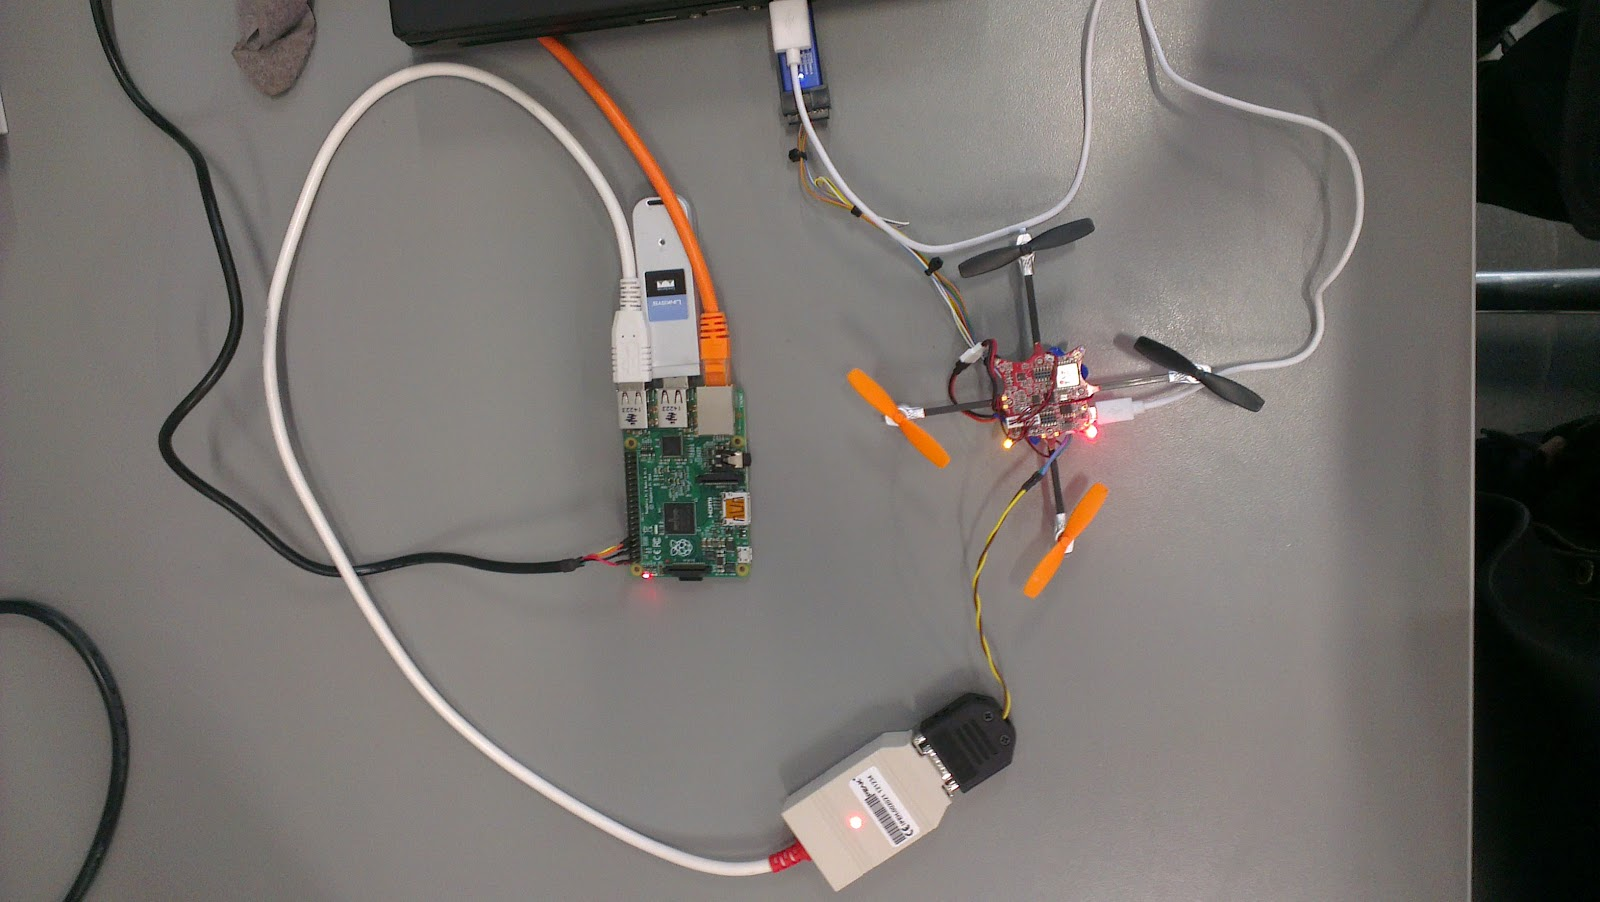
\includegraphics[width=0.6\textwidth]{graphics/test_test_setup_hw.jpg}
  \label{fig:boat1}
  \caption{Test-setup shown}
\end{figure}


The Rpi is connected directly to the PC using the orange ethernet cable.
The rosbag was stored and played on the PC, so the ethernet cable were used to share rostopics between the PI and the PC. The roscore where running on the PC.\\
The Ladybird drone is connected to the RPI using a PEAK CAN-adapter to transfer CAN messages. The Ladybird is powered by the white USB-cable and to show the position of the drone in QgroundStation. The PC is connected to the drone using ST-Link SWD to easier start, stop and restart the drones firmware during the test. To access a \ac{TTY} on the PI, an FTDI cable has been connected to the PC.


In order to obtain GPS-testdata to spoof into AQ, a rosbag was used to record data collected by the GPS mounted on the authors laptop. The setup can be seen in figure \ref{fig:test_laptop_and_gps} 
\begin{figure}[H]
    \center
    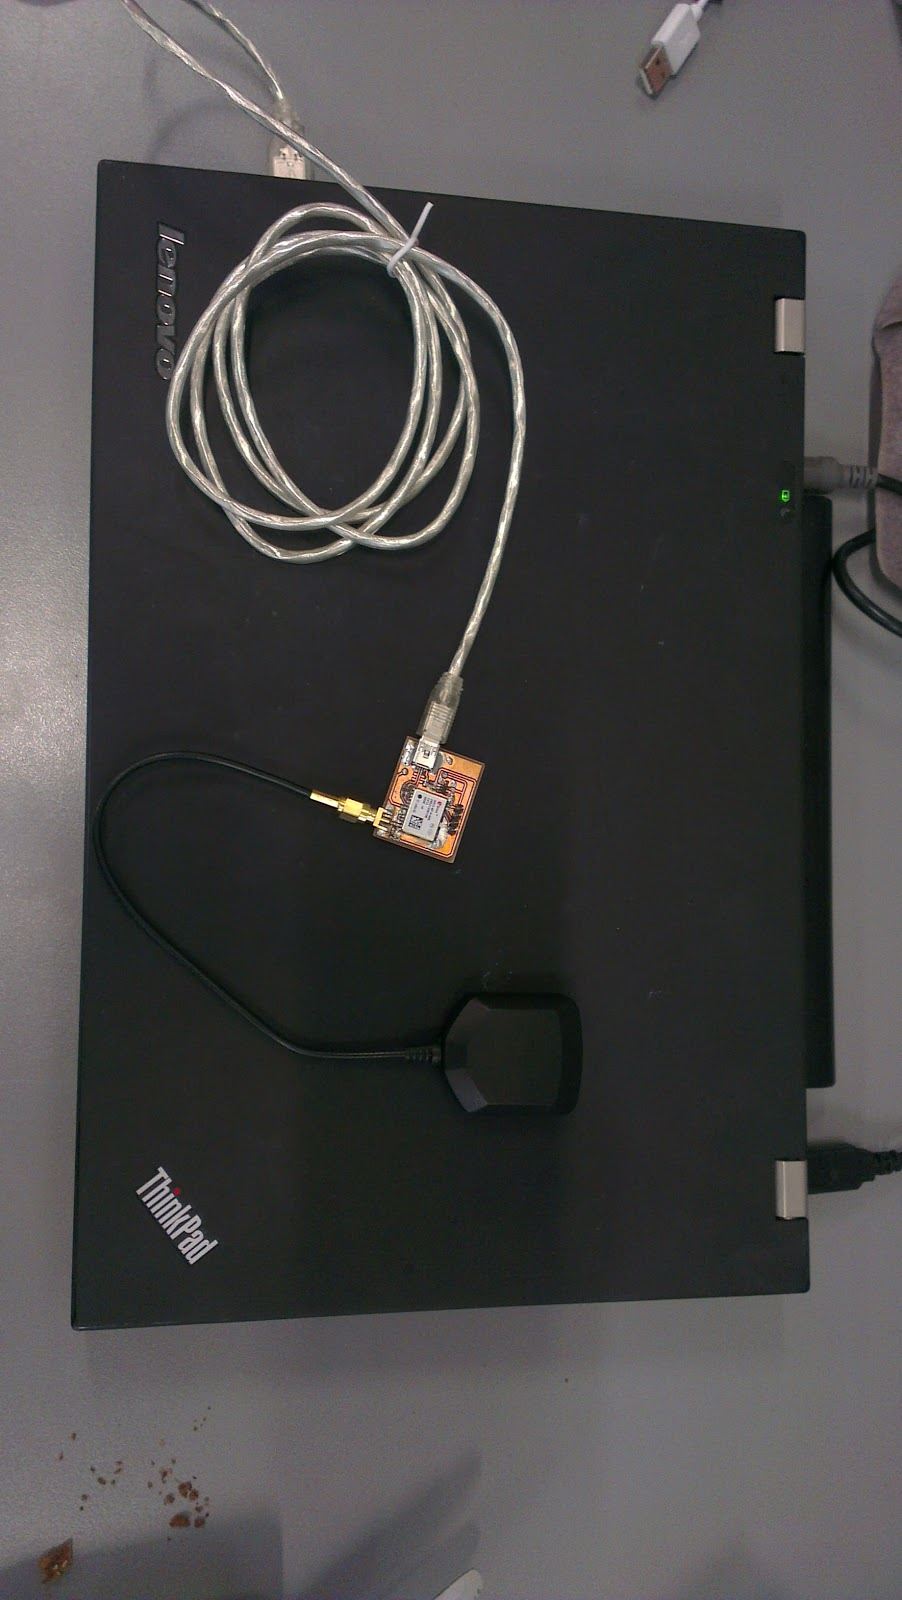
\includegraphics[width=0.5\textwidth, angle=90]{graphics/test_laptop.jpg}
  \caption[Comment]{The Neo6-P GPS (PCB developed by SDU), u-blox active GPS antenna \protect\footnote{ANNMS005} and authers laptop used in this test}   \label{fig:test_laptop_and_gps}
\end{figure}
The coordinates recorded by the rosbag is shown in figure \ref{fig:gps_raw_plot}. 
FreeNMEA\footnote{http://freenmea.net/} was used to plot the GPGGA messages obtained from the GPS.
\begin{figure}[H]
    \center
    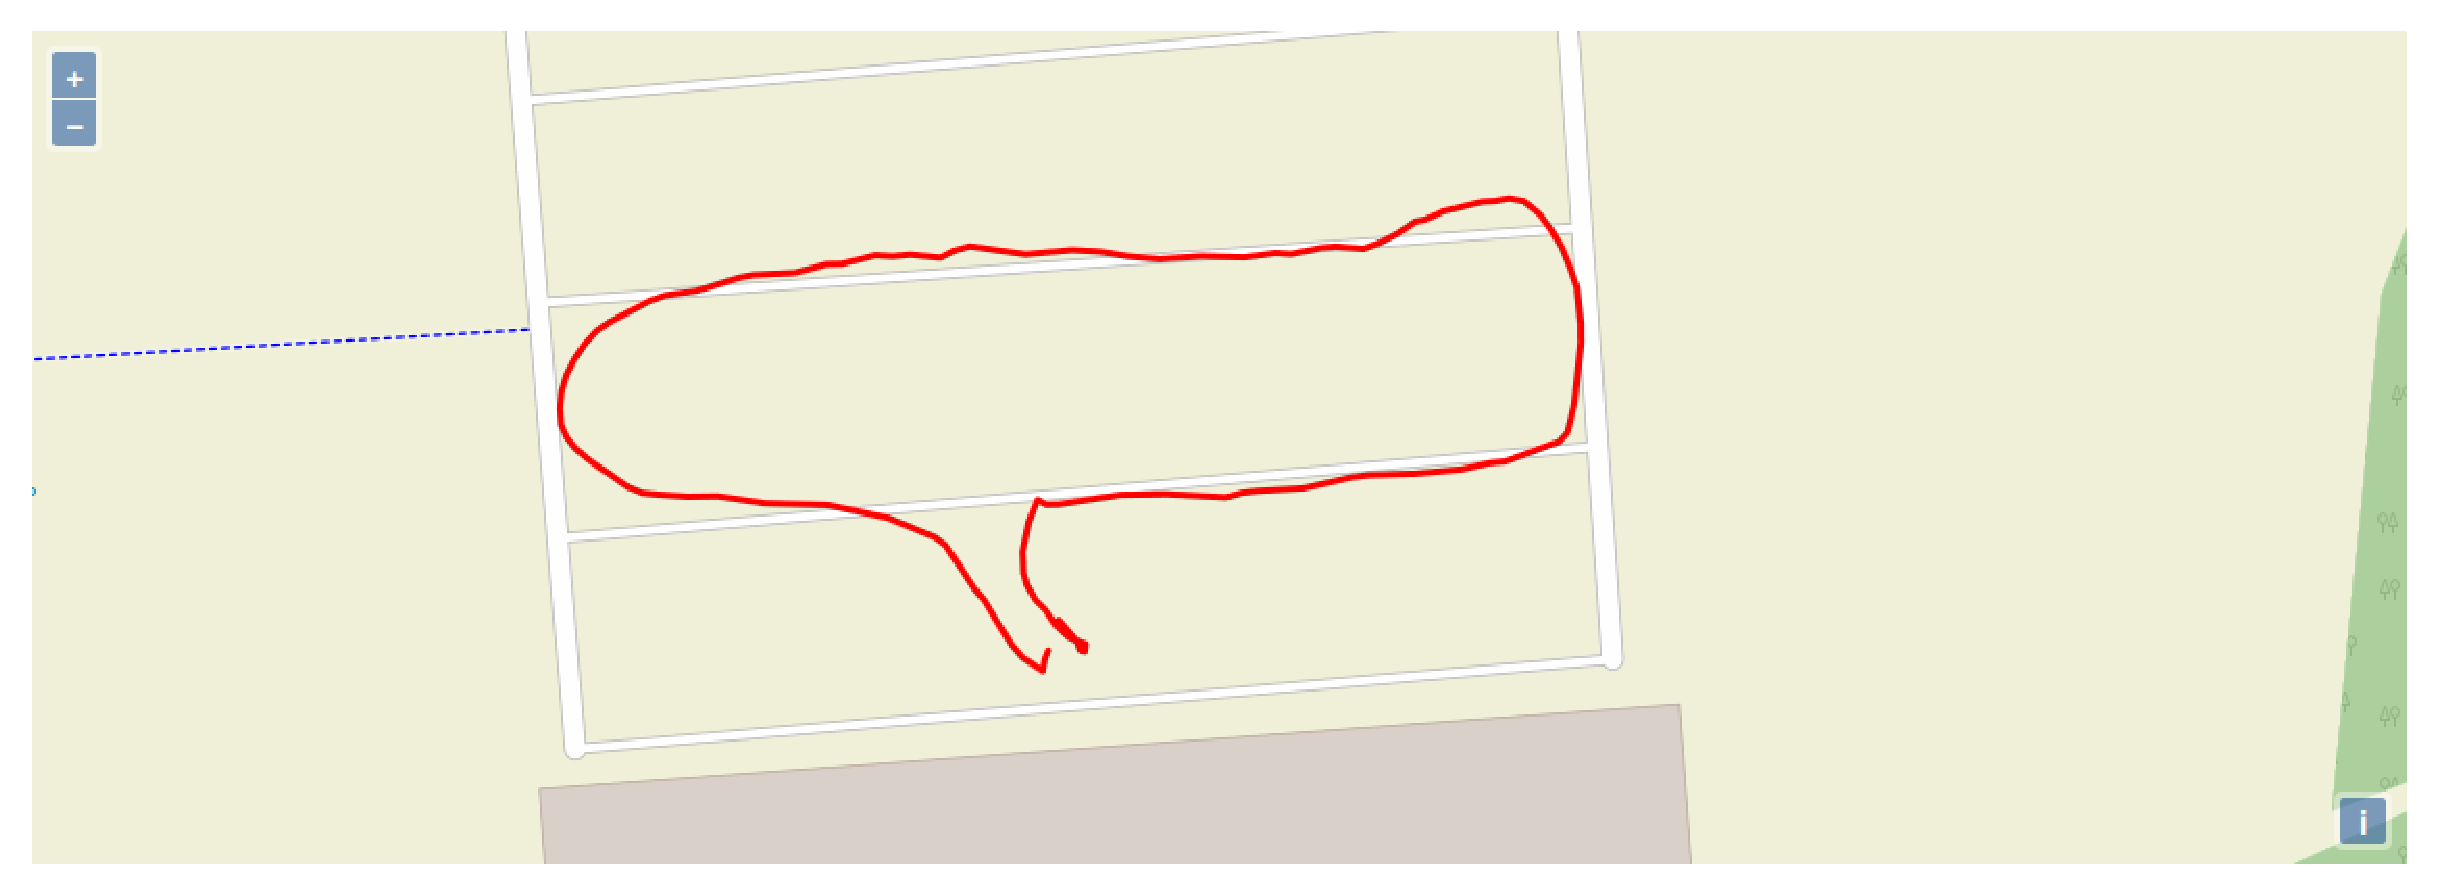
\includegraphics[width=1\textwidth]{graphics/gps_test_gps_plot}
  \caption{Test coordinates plotted}  \label{fig:gps_raw_plot}
\end{figure}
The rosbag containing the GPS coordinates where played on the Rpi, to see if the ROS node responsible for converting GPGGA messages into CAN messages were working. QgroundStation plots AQ's belief in where the drone is. The plot can be seen in figure \ref{fig:test_qground_plot}

\begin{figure}[H]
    \center
    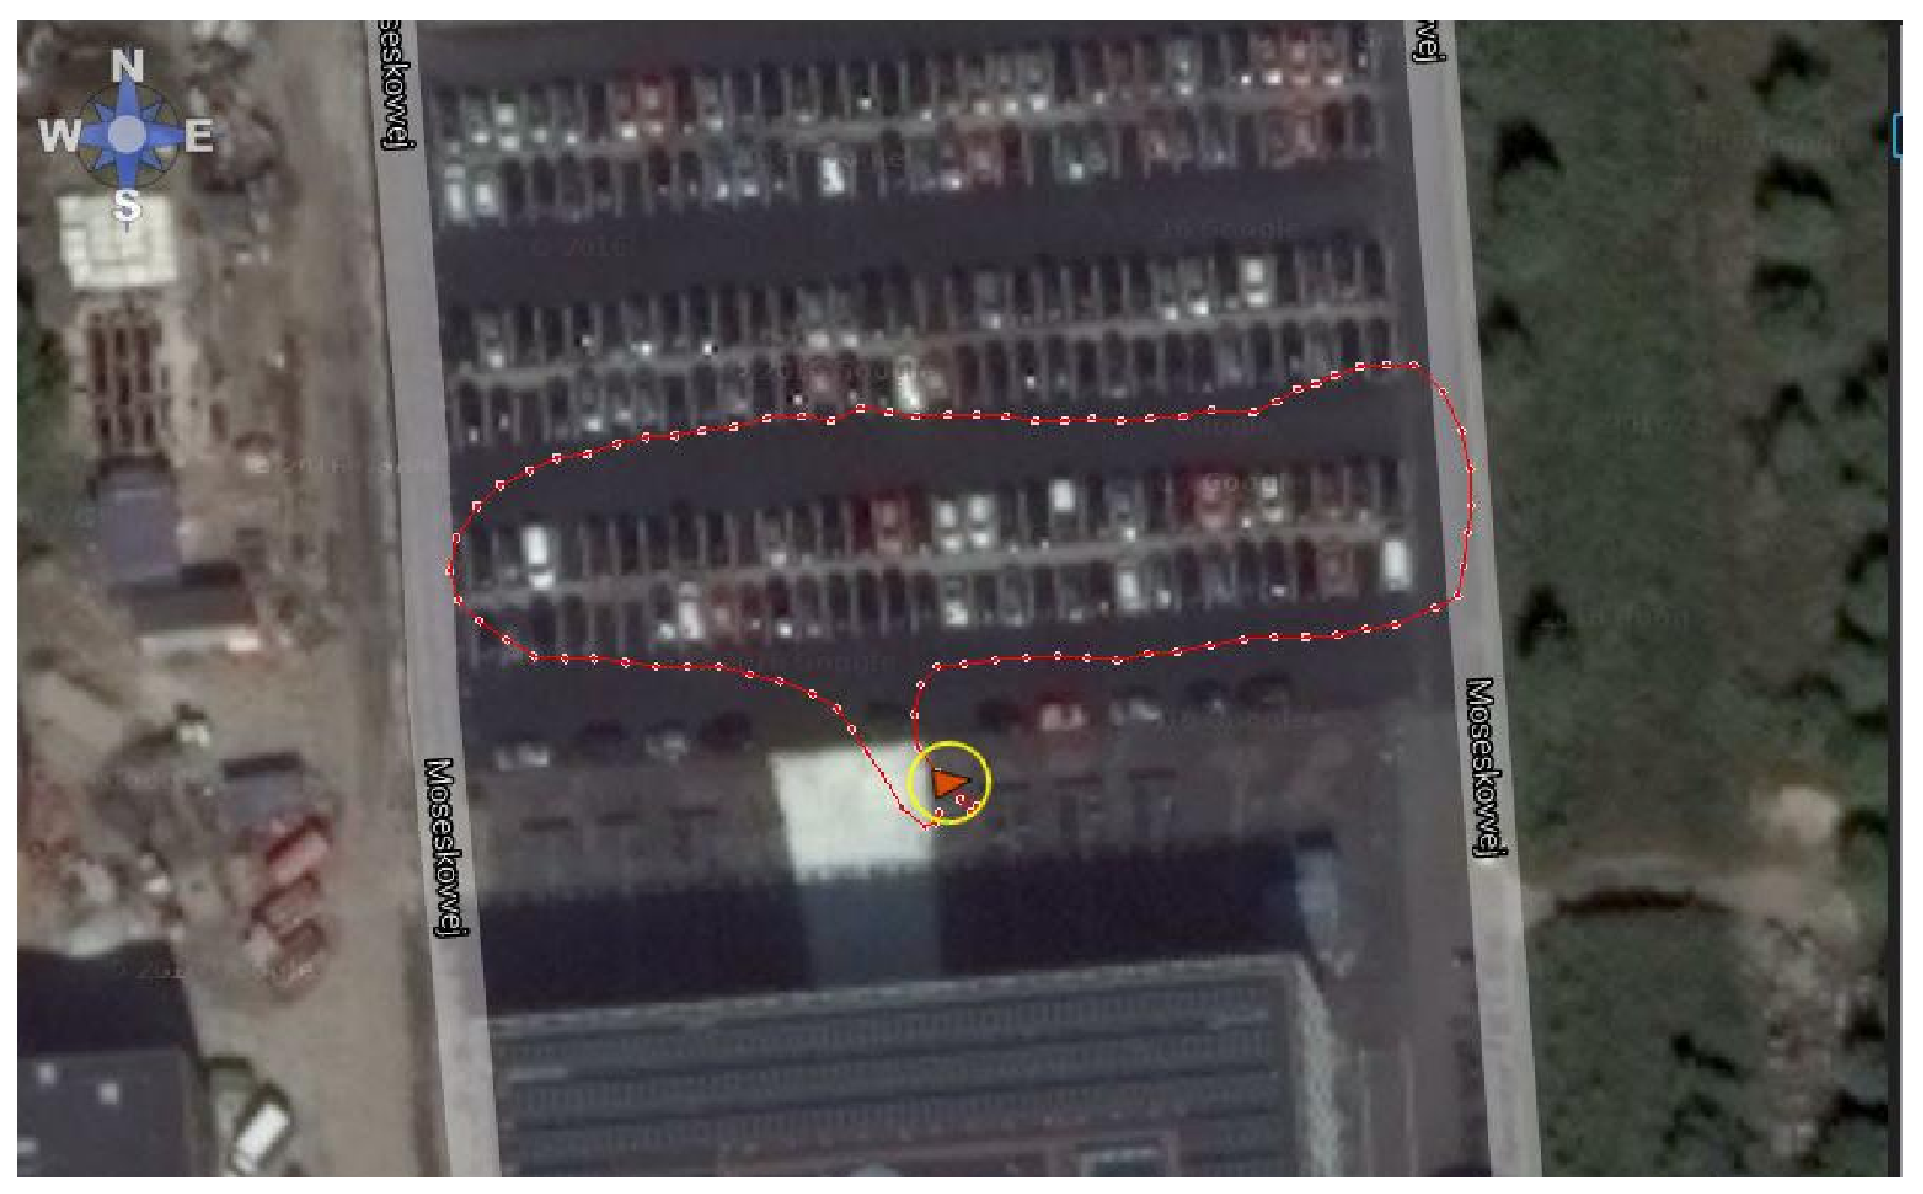
\includegraphics[width=0.8\textwidth]{graphics/test_qground_plot.eps}
  \caption{QgroundStations plot of AQ's belief in where the drone is}   \label{fig:test_qground_plot}
\end{figure}

\textbf{Conclusion}
This test visually confirms that the coordinates is spoofed correctly and read probably by AQ as long as the drone is laying on a table. Passing this test means there is reason to believe that it also works when the drone is airborne.


